\chapter{Methods}
In addition to the deployment of existing methods to achieve my research goals, this dissertation contains a number of innovations which are best described as methodological.  I include some of these innovations here, especially those of an extremely technical nature.  Some other methodological innovations, especially those of more interest to the computational neuroscience community, are reported later in the Results chapters.

\section{Approach to optimization using NeuronUnit}
Model optimization follows the following basic approach:
\begin{enumerate}
	\item Identify a model class whose parameters are to be optimized, e.g. the Izhikevich model.
	\item Identify a neuron whose experimental data will be used to guide optimization.
	\item Identify a suite of tests that can use that experimental data to guide the optimizer.
	\item Execute optimization of that model class against that suite of tests to return an optimized model.
\end{enumerate}
Within these steps are also a number of smaller decisions, including where the experimental data will be obtained and what kind of simulator will be used to run the model.
Using NeuronUnit, the steps above take the follow pseudo-code form:
\begin{lstlisting}[language=python]
# Import code from NeuronUnit
from sciunit import TestSuite
from neuronunit.models import MyModelClass
from neuronunit.tests import MyTestClass1, MyTestClass2, MyTestClass3
from neuronunit.data import get_data_from_database_x

# Get data about my  neuron
neuron_type = "Russell's neuron" # Replaced with a real neuron type in production
neural_data = get_data_from_database_x(neuron_type)
test1 = MyTestClass1
test_suite = TestSuite([test1, test2, test3])
\end{lstlisting}

%\section{Approach to Optimization using NeuronUnit}
Model optimization follows the following basic approach:
\begin{enumerate}
	\item Identify a model class whose parameters are to be optimized, e.g. the Izhikevich model.
	\item Identify a neuron whose experimental data will be used to guide optimization.
	\item Identify a suite of tests that can use that experimental data to guide the optimizer.
	\item Execute optimization of that model class against that suite of tests to return an optimized model.
\end{enumerate}
Within these steps are also a number of smaller decisions, including where the experimental data will be obtained and what kind of simulator will be used to run the model.

Using NeuronUnit, the steps above take the follow pseudo-code form:

\begin{lstlisting}[language=python]
# Import code from NeuronUnit
from sciunit import TestSuite
from neuronunit.models import MyModelClass
from neuronunit.tests import MyTestClass1, MyTestClass2, MyTestClass3
from neuronunit.data import get_data_from_database_x

# Get data about my neuron
neuron_type = "Layer 5 pyramidal Neuron"
neural_data = get_data_from_database_x(neuron_type)
test1 = MyTestClass1(observation=neural_data)
test_suite = TestSuite([test1, test2, test3])
results = test_suite.optimize(model)
\end{lstlisting}

There are two different paradigms for evaluating models in NeuronUnit. Under the first paradigm the model is supported by NeuronUnit, and dynamic simulations of the model are present on the host computer and can be efficiently re-run.

Under the second paradigm the NeuronUnit version of the model only consists of model inputs and outputs that are streamed as needed from a different environment. This may be the case due to the complexity of the model, where re-implementing the model would not improve clarity. Or the full model may exist on a remote machine with outputs accessed via an API. 
%Another way of saying this is that if a "model" is simply a digitized set of waveforms, converting it to a model is as simple as labeling things such that NeuronUnit and the scientist are both consistent about what is a model and what isn't. 
The optimization procedures I describe in this work involve both paradigms, where optimizing within the second paradigm required dedicated code that is not supported within the previously described frameworks.

\section{Model Class Implementations}
Because optimization may involve an extremely large number of independent simulations of the same class of model, each varying only in model parameter values, it is critical that both the overhead for model instantiation and the duration of simulation be as low as possible. We built faster Python implementations of two neuronal models -- the Izhikevich model and the adaptive exponential integrate and fire model. My implementations of the Izhikevich model was based on an existing MATLAB forward Euler implementation, while my implementation of the adaptive exponential integrate and fire model came from vectorized Python code, which was relatively slow.

I was able to use a tool to make both of these models perform faster than the standard versions for the brian2 and NEURON simulators. This tool, \cite{numba}, enables Just In Time compilation (JIT).
 %Without over stating things, 
 When regarding this thesis effort and its contribution to knowledge, some of the value to the neuroscience modelling community comes from the implementation of these two fast Python neural model simulations. Because these simulations are written in Python, the code that implementations them is easy to understand share and execute, because the models are fast to dispatch they are useful in both network and optimization contexts where performance is critical. 
 
%A component of this work the Izhikevich model, I plan to push to the Open Source Brain %\href{https://github.com/russelljjarvis/IzhikevichModel.git}

\subsubsection{Why Existing Approaches Were Not workable}
In this research effort significant time was spent shoe-horning pre-existing tools into an optimization frame work, with limited success. These tools included:  PyNN, brain2, \emph{NEURON}, jNeuroML-2. However, several unexpected road blocks were encountered on the way.
 
When applying reduced models to optimization, there was a cluster of known errors and limitations in pre-existing community standard reduced model simulators. 

To make optimization of models tractable it was important to do ongoing feasibility testing. For example its important to evaluate the the utility of established model implementations, as using these models to optimize may not in fact be feasible.\\ 
Despite an a large number of choices of FOSS reduced model implementations, many off the shelf implementations were not useful, or significant intervention was required to make some established implementations workable inside an optimization framework. \\
 
Some revisions to the Izhikevich model include equation tweaks, in order to let cells better reproduce in-vivo firing dynamics, such as bursting, and re-bound spiking \url{https://github.com/OpenSourceBrain/IzhikevichModel/blob/master/MATLAB/izhi2007.m}. However, when multiple equations, however closely related, are incorporated under the same umbrella, this fractures the implementation of the model into sub-models. The \emph{NEURON} implementation of the Izhikevich model is fractured. There are different implementations for different regimes. This meant that switching between model regimes during optimization would be a non-trivial exercise because the is already splintered between two languages (NEURON, NMODL, python), the source code would be highly complicated such that it would not be readable, and it would loose generality, overly customized towards one target model. The NEURON code, needed NMODL files to be compiled for each different regime, and promised performance of the C based NEURON library was not actualized. The only benefit to using this model, was that its parameter ranges are well tested and understood within OSB and NeuroML-2 community.

Because the PyNN implementations of the Izhikevich models are "wrapped" versions of essentially NEURON models, PyNN models still retained the disadvantages of the NEURON models (surprisingly poor speed on the Izhikevich model) while introducing other problems. PyNN is designed to preference the description and implementation network simulations. A data-type called a "lazy-array" is the smallest elemental container for neuron models in PyNN, but it is meant to store populations of neurons as opposed to single neurons, as such the lazy-array often slows down and gets in the way of the single neuron simulations, which model fitting depends on.
%(lazy array evaluation). 

 Sub models $[1-3]$ are really different parameterizations of the same equation, sub-models $[4-7]$ are actually different equations, meaning that there is a total of $4$ Izhikevich sub-models. To permit optimizer access to the broadest range of Izhikevich dynamics, a new meta-parameter $cell_type$, was created. This number ranging $[3-7]$ (unique model equations included only), allows the optimizer to change which Izhikevich sub-model it samples from. Later in on in results, we see that in fact even when fitting to static electrical properties, optimizer access to the broader set of firing regimes improved the quality of fits.


%The described limitations of the 
%https://github.com/NeuralEnsemble/PyNN/issues/370$%}, journal={GitHub}, author={Davison A}
%}


%@misc{neuralensembleadexp, title={pyNN.neuron %implementation of AdExp is unstable, gives poor results  Issue $#266 · NeuralEnsemble/PyNN$}, url={$https://github.com/NeuralEnsemble/PyNN/issues/266$}, journal={GitHub}, author={Davison A.}
%}
\url{https://github.com/NeuralEnsemble/PyNN/issues/370} 
%\cite{neuralensemble_adexp}
\url{https://github.com/NeuralEnsemble/PyNN/issues/266} 
%\cite{neuralensemble_adexp2}
 
A constant error warning plagued brian2 investmentallations was.
\begin{verbatim}
Brian2 causes error:
 ERROR      Brian 2 encountered an unexpected error. If you think this is bug in Brian 2, please report this issue either to the mailing list at <http://groups.google.com/group/brian-development/>, or to the issue tracker at <https://github.com/brian-team/brian2/issues>. Please include this file with debug information in your report: /tmp/brian_debug_t0acbm4l.log  Additionally, you can also include a copy of the script that was run, available at: /tmp/brian_script_juzhsbph.py Thanks! [brian2]
Traceback (most recent call last):
\end{verbatim}
In two classes of model a feasible choice of implementation did not exist and it was easier to re-implement those models. The two models I re-implemented were
the Adaptive Exponential Integrate and fire Model, and also the IZHI
model.  In the work below, I profile existing model implementations, and
justify the reasons for re-implementing.\\
\\
This is in contrast to the brian2/neuraldynamics AdExp model, which took
between 2 or 3 times longer to find a rheobase current injection value. However the slowness is not caused by the simulation backend (brian2 which is relatively fast and efficient). The slow down is caused by the way the model is defined. Specifically the
model is defined in a middle code layer neurodynamics \cite{gerstner2014neuronal}.\\
\\
It is very likely, that the model implementation is correct, since Gerstner is an author of one of the original adaptive exponential publications, and the neural dynamics book that the brian2 code is strongly affiliated with. Since Integrate and Fire models don't formally include spikes when an implementation does include spikes, it is an optional add on.\\
\\
The AdExp neurodynamics models default implementation causes spikes with peaks below $0mV$, since the IZHI model like all integrate and fire models do not explicitly include spikes\\
\\
This is not technically wrong, but it violates
assumptions in the \emph{NeuronUnit} feature extraction protocol. The default spiking behavior, looks odd, and it is simply this poor model definition that is causing a slower optimizer performance. The optimizer takes an unusual waveform shape, and searches for longer in distant
parameter regions to find a good fit.\\
\\
Over the course of evaluating the brian neural dynamics model \cite{gerstner2014neuronal}. I experienced some phenomena that only occurred in the context of genetic algorithm optimization. The reason why optimization provides a different evaluation context is because, in optimization simulation objects are required to be created and destroyed rapidly and on mass. Brian2 is designed to be an efficient network simulator, the case of being designed for network simulation, may assume you will want to create a lot of neural models that persist efficiently together in memory (this was also a problem with PyNN models). Therefore you might see below, that while only one brian model exists in memory, performance is okay, but when creating and destroying models rapidly and on mass a slow down occurs.\\
\\
Below I have implemented a Python integrator for the adaptive exponential integrate and fire model. This solver led to faster evaluations of current injection experiments. The integrator I developed has a $0mV$ spike when evaluated at default parameter values.\\

Brian2 and SciUnit sometimes collided in name space and logging.
%\href{https://github.com/scidash/sciunit/pull/124/files/83907ba68740642178ebb91084f6e382e06a43c4#diff-d68791d2ed5dfaa96a900be6180bd950}

\section{Profiling the JIT Enabled AdExp Model}
Mean time taken on single model evaluation:$ 0.0012554397583007812s $
Mean time taken to compute Rheobase:
$0.183s $
This was slightly faster than Izhikevich implementation which was for total rheobase solution $ 0.462s $ and $  0.002 s$ per run. Solving for Rheobase takes a average of 15 model evaluations.
%\begin{figure}    
%\begin{center}
%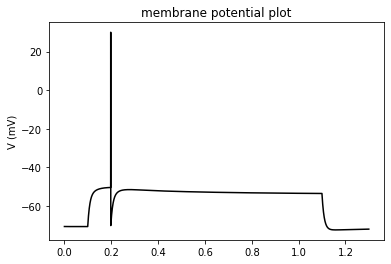
\includegraphics[width=0.25\linewidth]{figures/backend_check_files/backend_check_6_2.png}
%\caption{}

%\end{center}
%\end{figure}

%\begin{verbatim}
%    251 ms +- 5.02 ms per loop (mean +- std. dev. of 2 runs, 1 loop each)
%    240 ms +- 11.1 ms per loop (mean +- std. dev. of 2 runs, 1 loop each)
%    223 ms +- 12.5 ms per loop (mean +- std. dev. of 2 runs, 1 loop each)
%\end{verbatim}

\begin{verbatim}
    922 ms +- 12.7 ms per loop (mean +- std. dev. of 7 runs, 1 loop each)
\end{verbatim}

\subsection{Comparison of Parallel and Serial Speeds and Accuracy}

Below is the Brian2/NeuralDynamics AdExp model. In-order to make the spike height greater than $0mV$ it was easier to use computer code to schedule waveform modifications that occur straight after the the brian2 simulation, these scheduled waveform modifications can be considered part of a peripheral shell of simulation code. In postprocessing
the waveform data type is a Neo Wave form object that is artificially the algorithm of determining rheobase and displaying results. The time of this model is determined on multiple factors, as discussed elsewhere, execution time is not uniform across model parameterizations. Models with multispiking behavior will take longer to solve.

Simulation times for this model vary, dramatically possibly because of
lazy evaluation, the simulation times may vary according to what else
you are running on your computer. Not all models experience a speed up when executed in parallel, however
this model was faster in the parallel Rheobase determination algorithm. Some common times are: $3.92,6.75,4.48,5.17$. Mean time was:

\subsection{Comparison of Time to Find Rheobase}

Custom implementation JIT enabled implementation: $4.0s$. 
Brian2 taken to find Rheobase: $4.40s$ (serial), $3.976s$ (parallel).

The evaluation times between Brian2 and the custom written
integrator are similar. Both have average rheobase solution times of approximately 4 seconds, however the spike shape derived from the custom written integrator look more realistic under default paramaterizations. The biological plausibility of default model paramaterization has consequences for model optimization speed, because when  models undergo mutation and cross-over the mean of random models regressors towards the default model initialization, and if the default model is a bad fit to data, the average model sampled by the genetic algorithm will also be bad to data.\\

\begin{figure}
\centering
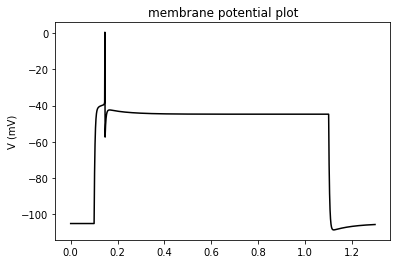
\includegraphics[scale=0.45]{figures/backend_check_files/backend_check_12_10}
\caption{Model Parameterization of the brian2 Simulator with the customization: interpolated spike height, forced to be above $0mV$}
\label{fig:sub1}
\end{figure}

\begin{figure}
\centering
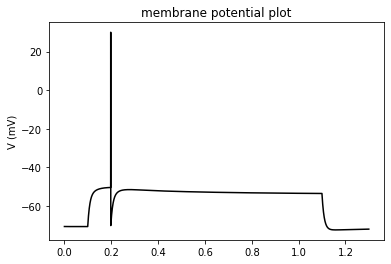
\includegraphics[scale=0.45]{figures/backend_check_files/backend_check_4_2}
\caption{Default model parameterization of the custom written integrator}
\label{fig:sub2}
\caption{Comparison between two Adxaptive Exponential Implementations}
\label{fig:test}
\end{figure}




    
$272 ms +- 66.5 $/mu$s per loop (mean +- std. dev. of 2 runs, 1$ loop each)

The next model to be evaluated is the NEURON Izhikevich model. The NEURON Izhikevich model has various draw backs. 1. It depends on an external file which must be recompiled each time this project is recreated. 2. The build environment of NEURON is non-trivial, and only a super dedicated NEURON modeller would install it on their system. Any performance advantage of using NEURON investment does not exceed the installation cost of installing the program. 3. The model implementation code is less generalizable than than the published Izhikevich model itself. Where the standard NEURON-NeuroML code only covers the Regular-Spiking model * This is likely due to a name space conflict between Capacitance. Neuron has a `capacitive' mechanism inside modelled Neurons, this particular model has section capacitance as well as an introduced capacitive term inside a C-compiled mechanism. Both contribute to a the membrane
potential calculation. * The NEURON Izhi model took $78$ seconds to find the rheobase current injection value $ 51.79367065 * pA $.

    
%\begin{center}
 %   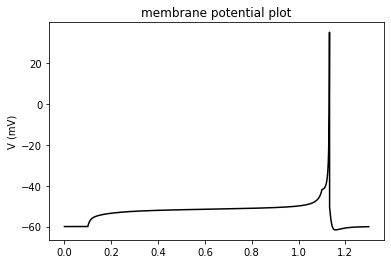
\includegraphics[width=0.7\textwidth,]{chapters/figures/backend_check_files/backend_check_14_2.png}
%    \caption{where is picture}
%\end{center}


%\begin{figure}
%    \centering
%    \includegraphics{chapters/normal_distribution}
%    \caption{This is your image%}
%    \label{fig:my_label}
%\end{figure}
%A tool numba JIT

% https://www.overleaf.com/learn/how-to/Images_not_showing_up 

        
The enabled forward Euler python Izhikevich model was very fast. The forward euler
implementation utilized Numba JIT \cite{lam2015numba}. Rheobase is found in under a second,
and in many cases close 0.5 seconds. This represents a very dramatic
speed up. Unlike the NEURON NeuroML implementation of the izhikitich equation,
this implementation is just as generalizable as the original MATLAB
implementation of the Izhikevich model, because it was possible to unify the fractured implementations in the one python simulator backend.

\subsection{NEURON+Python single compartment Conductance Model.}

Conductance based models took approximately the same amount of time to evaluate the Rheobase search algorithm as the python implementation.

The author also engineered GLIF model support for $NeuronUnit$ tests. In practice these models where hard to configure without expert knowledge, GLIF models contain the most parameters of all models, and many of these parameters are multi dimensional. GLIF models do not by necessity spike, interpolated spike times, are added in however, it does not make sense to evaluate GLIF models on spike shape features.

It is worth noting that the layer 5 neocortical pyramidal neuron was very slow to dispatch relative to the reduced models developed in this thesis work. Where as a typical reduced model described here evaluated in the order of $2.5 ms$, this model on average took $5.74$s, for a single run and $34.8$s to solve for the models Rheobase, current. To be fair, the model was run without activating NEURONs variable time step cvode. However, even with variable time step applied to the differential equation solver the magnitude of the disparity is still still several $seconds:$ several $ ms$. 

% time taken to compute rheobase $ 12.6s $


%\begin{verbatim}
%  time taken on
%  block 0.6859951019287109 \textbackslash{}n3.3 ms +- 9.79 %$\mu$s per loop (mean +- std. dev. of 2
%  runs, 100 loops each)\textbackslash{}n3.32 ms +- 30.9 us per loop (mean +- std. dev. of 2 runs,
%  100 loops each)\textbackslash{}n3.19 ms +- 10.9 us per loop (mean +- std. dev. of 2 runs, 100
%\end{verbatim}
        


%This problem in the default parameterization of the python model was later located in the scale or units of capacitance, if default capacitance parameterization is multiplied by 100.0 the problem goes away.


%\begin{center}
%\includegraphics{figures/backend_check_files/backen%d_check_22_2}
%\end{center}

%$ 1.40762329 * pA $


% \subsection{NEURON versions of single compartment Conducance
% model.}

% Took $8.57$ seconds to find Rheobase.

%Hodgkin Huxley Conductance based channels models took approximately the same amount of time to evaluate the Rheobase search algorithm as the python implementation.

%The NEURON implementation was slightly faster, and the default parameterization of the model lacked `ringing'', or below threshold oscillations that the Python ODE version had under default conditions.

%This problem in the default parameterization of the python model was later located in the scale or units of capacitance, if default capacitance parameterization is multiplied by 100.0 the problem goes away.


%which makes debugging their behavior very difficult. %None the less GLIF models where among the fastest to evaluate, and the author had success in making fitting these models to Allen Rheobase data.

    %\graphicspath{ {../figures/} }
%    \begin{center}
%    \begin{figure}
%    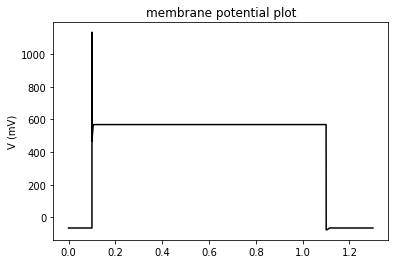
\includegraphics{figures/backend_check_files/backend_check_26_2}
    %kend_check_files/backend_check_26_2.png}
%    \end{figure}
    
%    \end{center}
%\begin{verbatim}
% 112.5 pA
%'value': array(1.40645904) * pA
%\end{verbatim}

% parameters of an adaptive exponential model
%\begin{verbatim}
%\{'El\_reference': -0.07016548013687134, %'C': 3.990452661875942e-10%,
%'init\_threshold': 0.02964956889477108, %'th\_inf': 0.02964956889477108,
%'spike\_cut\_length': 109.5, %'init\_voltage': -35.0, 'R\_input': %910258965.9792937\}
%\end{verbatim}
%$ Rheobase = 112.5pA $
%time taken to execute GLIF model when deliberately undersampling to save time.
%$ 0.23476457595825195 $

    


%$ 112.5 pA $
%$0.0 mV$ $-0.065 mV$

%    \begin{verbatim}
%    \{'value': array(183.33333333) * pA\}
%    \end{verbatim}

%\begin{verbatim}
%array(112.5) * pA
%\end{verbatim}


%\begin{verbatim}
%    0.017240506310425608 mV -0.08583939747094235 mV
%    0.017240506310425608 mV% -0.08583939747094235 mV
%\end{verbatim}

    %\begin{center}
    %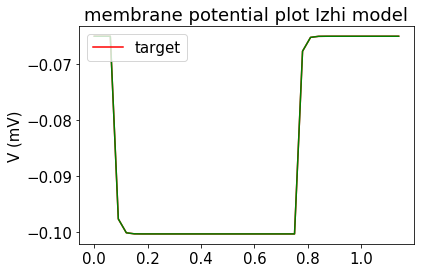
\includegraphics{figures/backend_check%_files/backend_check_32_2.png}
    %\end{center}

%\input{chapters/methods/rheobase}

\section{Pre-Existing Model Class Implementations}
First I accessed an implementation of the Izhikevich model that was translated from jNEUROML into a NEURON simulator implementation.
However, this implementation fragmented the family of Izhikevich models into chattering and non-chattering subtypes.
The model implementation also seemed to have an internal conflict between two capacitive terms and could not reproduce all of the original publication figures.
Although the NEURON simulator is designed to be fast, there is a cost associated with reloading the NEURON environment many times in fast succession, and implementation odel execution times were not brief enough to be useful for optimization.

\section{Other Model Class Implementations}
For various reasons described in detail below, existing implementations of some models were not adequate for this research.
These reasons included speed, generality, and consistency.

\subsection{Model Execution: The Need for Speed}
Because optimization may involve an extremely large number of independent simulations of the same class of model, each varying only in model parameter values, it is critical that both time costs--both the overhead for model instantiation and the duration of simulation itself--be as low as possible.
Existing modeling tools contain overhead associated with model initialization and shuttling results in memory.
These costs are trivial for single simulations, but begin to add up in optimization runs of thousands or even millions of simulations.  
Even the marginal cost of simulation--expressed as seconds on a wall clock per seconds of model output simulated--is often slower than expected using existing tools, due to some of these tools being written to accommodate more complex, biophysical models, rather than engineered for raw speed.
During optimization, many parameter sets are explored, and the speed of  simulation can be determined by the parameter values.
For example, those parameter sets which produce many spikes in a given simulation run more slowly, because $\frac{dV_{M}}{dt}$ changes rapidly throughout the simulation, necessitating reductions in simulation step size to avoid numerical instability.

\subsection{Model Design: Lack of Generality}
Significant time was spent in the early years of this project shoe-horning pre-existing tools into the desired optimization framework, with limited success.
These tools included, among others, model designers and neural simulators such as PyNN, Brian2, NEURON, and jNeuroML.
However, several unexpected road blocks were encountered on the way.

\subsubsection{NEURON}
The NEURON simulator is a very mature and respected neuron and neural network modelling framework \citep{carnevale2006neuron}. This simulator specializes in multi-compartment conductance based models of neurons and neuronal networks, but the simulator has also been made to accommodate many reduced model implementations. The NEURON implementation of the Izhikevich model is fractured in that there are different NEURON NMODL implementations of the equations for different parameter regimes.

When running only a single model simulation this is not much of a problem. However, switching between Izhikevich model regimes during optimization (as would occur when a parameter value crossed a regime boundary) is a non-trivial exercise.
Even if successful, any multi-language source code successfully implementing this would be complicated, unreadable, and lack generality.
Specifically, NEURON requires NMODL files to be compiled for each different regime, and it may be difficult to know in advance which regimes the optimizer is likely to sample from.
Additionally, the promise of fast performance due to the C-based NEURON library is not actualized with this model.
Because NEURON is well-understood within the OSB and NeuroML community, I used it only to produce reference simulations to verify that the output of my model implementations were in fact accurate according to community standards.

\subsubsection{PyNN}
PyNN provides the convenience of working in Python, and with a convenient procedural interface for model design and execution \citep{davison2009pynn}.
However, its implementations of most reduced models (e.g. Izhikevich) are simply ``wrapped" versions of NEURON models; consequently PyNN has the same disadvantages as NEURON.
PyNN is also designed with network simulations in mind, which means its designers have chosen performance trade-offs that favor network simulations over single neuron simulations.
For example, a data-type called the ``lazy-array" is the most elemental container for neuron models in PyNN, but it is meant to store populations of neurons as opposed to single neurons;
as such the lazy-array adds overhead to accessing single model results.

% in slow single neuron simulations.

Additionally, the NEURON implementations that underlie the PyNN-provided AdEx and Izhikevich model classes suffer from some fidelity issues under certain regimes and parameter sets, compromising optimization quality (see \cite{neuralensembleadexp2, neuralensembleadexp} for details).

\subsubsection{Brian2}
Brian2 \citep{stimberg2019brian} is, in principle, an excellent simulator for working with reduced neuron models, as it allows for differential equations to be expressed in an intuitive form, while also keeping track of dimensions and units.
However, it may not be mature enough for complex applications, as it produced errors in optimization contexts that did not occur during routine simulation of single-parameter sets.

Even when these errors did not occur, (e.g. using the Brian2 AdExp model), certain optimization steps (such as identifying the rheobase current for a given set of model parameters) took 2-3 times more simulation time then a reference approach (described in the next section).
This slowness was not caused by the simulation mechanics themselves (Brian2 is relatively fast and efficient, as described in \cite{stimberg2019brian}.)
Instead, these delays are caused by the way the model is internally defined, specifically using a
so-called ``neurodynamics" layer \citep{gerstner2014neuronal}.

While it is very likely that this implementation is useful and correct in many contexts (Gerstner is an author of one of the original AdEx model publications \citep{brette2005adaptive}, and the Brian2 implementation is derived directly from his work), it is problematic for the feature extraction step required in optimization.
Specifically, these implementations do not formally contain any notion of ``overshooting" spikes, since when the spike threshold is reached, the membrane potential is simply set to some reset value; the presence and timing of a spike is recorded only when a separate process is explicitly set to watch for such an event.
This is not technically wrong, but it violates a key assumption in the \emph{NeuronUnit} feature extraction protocol (the existence of an action potential waveform to extract), and the extra layer for detection of spiking adds computational overhead.
Imputing a spike-like waveform near threshold can help solve the problem, but then optimization results and performance becomes contingent on the design of this waveform imputation, and not on the model itself.

Lastly, over the course of evaluating the Brian neural dynamics model \citep{gerstner2014neuronal}, I encountered some problems specific to genetic algorithm optimization.
This context is not identical to simply running a series of simulations in series, because optimization operates in parallel, must fit into computer memory, and thus requires that simulation objects be created, simulated, and then destroyed rapidly and en masse.
Since Brian2 was designed for stability, is was not designed to make model disposal computationally efficient (the problem of clearing objects from memory efficiently is, from a computer science perspective, trickier than it might initially sound).
Therefore, performance of Brian2 suffered when I re-purposed its code to work in an optimization context.
Brian2 does support its own internal scheme for model fitting \citep{brian2modelfitting}, however this scheme was only published late in this thesis work, and it is unknown what technical tricks they employed to enforce model garbage collection. 
Additionally this scheme is highly divergent from the multi-objective DEAP framework described in Section \ref{sec:tech-details}, so it is not readily interoperable with the model fitting workflow described here.

\subsubsection{My Approach}
\label{sec:new-models}
In summary, despite several choices for existing, free, open-source software (FOSS) reduced model
implementations, these implementations were not useful, or significant intervention would have been required to apply them within an optimization framework.
To overcome this and accelerate optimization, I built faster ``direct" implementations of two neuronal models (the Izhikevich model and the AdEx model).
One of the these was inspired from the existing MATLAB forward Euler implementation of the Izhikevich model, while the other was adapted from an existing Python implementation of the AdEx model using vectorized code.
While neither of these was especially fast, they provided the basic recipe upon which a faster Python implementation could be built.
Do note that the purpose of these new implementations was not model exploration, analysis, or sharing; existing tools are adequate for these purposes.
The purpose of the new implementations was simply to make large optimization runs computationally tractable.

Although typically much faster than R, Python does not have a reputation for speed; implementation details have a large impact on performance.
Therefore, I used a tool called Numba \citep{lam2015numba} that enables Just-In-Time compilation (JIT) of Python code, making it comparable in speed to compiled C code.
This tool cannot be applied to any arbitrary Python code, so functions to which it is applied must be designed with only a fairly plain subset of the usual syntax and library of Python.
In other words, it cannot be used to simply speed up any pre-existing Python code.
%all code is hand-coded, even cutting and pasting is done by hand suggested synonym crafted.
I crafted the two model types above to be JIT-compliant, with the result that both became significantly faster than analogous models using NEURON or Brian2 simulators.
Importantly, simulation outputs retained a binary near-match in all cases, confirming that nothing was lost in the course of gaining this performance improvement.
I used these new implementations extensively throughout the project, and they are available to others at \cite{jithub}. 
The code that implements them is fairly easy to understand, share, and execute, and I hope they may be useful to others who have similar performance needs, either for optimization contexts or in large network models on generic commodity computer hardware where small performance gains are worth chasing. 

Some models were executed in their native implementations using the NEURON simulator with an adaptive time step.
After each model run, the variable time step vectors were resampled into fixed time step vectors using interpolation.
I accelerated this inherently slow process by applying the JIT framework to prior code contributed by a colleague \citep{birgiolas2019towards}.

Below, I profile my implementations and compare them to the existing FOSS implementations.
My implementations led to faster per-simulation evaluations of simulations involving somatic current injection. 
Furthermore, my implementation exhibited over-shooting spikes (spikes crossing 0 mV, as occurs in real neurons), making them more compatible with NeuronUnit feature extraction.

\subsection{Profiling the Models}
Obtaining the rheobase of a model for a single parameter set requires simulating it many times at different values of somatic current injection until the minimum action-potential inducing current is obtained (to within some tolerance; here I used 0.1 pA, near the standard deviation of thermal noise).
This takes 10-15 simulations, on average.
\begin{verbatim}
My AdExp implementation:
Single model simulation: 0.00126 s
Rheobase computation: 0.183 s

My Izhikevich implementation:
Single model simulation: 0.002 s
Rheobase computation: 0.462 s
\end{verbatim}

\subsubsection{Comparison of Speed and Accuracy Versus Brian2}
In-order to implement NeuronUnit-compatible Brian2 AdEx model simulations, I imputed spike waveforms (at recorded spike locations) immediately following each simulation.
The simulation time of this model is determined by multiple factors, as discussed elsewhere. Execution time is also not uniform across model parameterizations; in particular, parameter sets exhibiting more spikes take longer to solve numerically.
I compared this with the same parameter sets in my implementation, with the results shown below:

A large fraction of the time spent simulating models under a single set of parameters is spent obtaining the rheobase current, upon which several subsequent tests and extracted features depend.

The JIT implementation of the AdExp model was approximately 1000$\times$ faster than the Brian2 model.
Another benefit of the JIT implementation was that it did not require imputation of action potential waveforms (as was required for the Brian2 implementation); without additional work, the JIT implementation produced much more realistic-looking action potential waveforms under most model parameterizations.
To the extent that action potential shape is an optimization target, this is a decisive advantage for the JIT implementation.

\begin{figure}[!htb]
\begin{center}
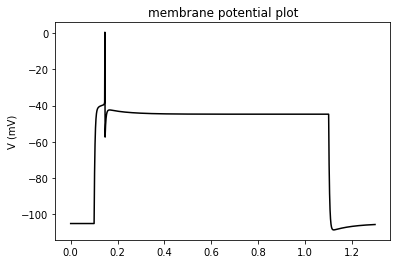
\includegraphics[scale=0.7]{figures/backend_check_files/backend_check_12_10.png}
\caption[Brian2 simulation of the AdEx Model]{\textbf{Brian2 Simulation of the AdEx Model.} Simulated membrane potential trace from the AdEx model at rheobase using the Brian2 simulator. The action potential waveform has been interpolated at the time when the simulator reported a spike.
The horizontal axis shows time in seconds.}
\label{fig:AdEx-Brian2-sim}
\end{center}
\end{figure}

\begin{figure}[!htb]
\begin{center}
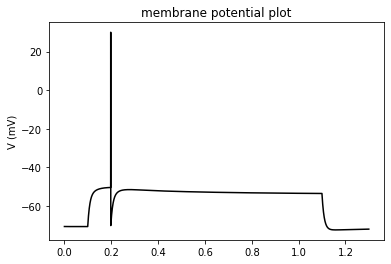
\includegraphics[scale=0.7]{figures/backend_check_files/backend_check_4_2.png}
\caption[JIT Simulation of the AdEx Model]{\textbf{JIT Simulation of the AdEx Model.} Simulated membrane potential trace from the AdEx model at rheobase using my JIT implementation. In contrast to Fig. \ref{fig:AdEx-Brian2-sim}, the dynamics of the action potential arise naturally from the integrated equations and do not require interpolation.}
\label{fig:AdEx-JIT-sim}
\end{center}
\end{figure}

\subsubsection{Comparison of Speed and Accuracy vs NEURON}
I also compared the performance of my implementation of the Izhikevich model to the one generated by NEURON from the OpenSourceBrain Izhikevich model NeuroML2 files.
This NEURON implementation has several drawbacks, including: 1) It depends on an external file which must be recompiled each time this project is recreated; 2) The build environment of NEURON is non-trivial; 3) The model implementation code is less generalizable than than the published Izhikevich model itself.
For example, the standard NEURON-NeuroML2 code only covers the Regular-Spiking flavors of this model, and does not support the full range of model parameterizations; 4) Name space conflicts between built-in NEURON parameters and Izhikevich model parameters.  

%\begin{center}
 %   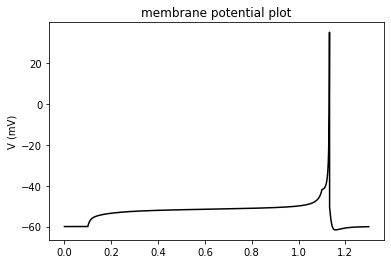
\includegraphics[width=0.7\textwidth,]{chapters/figures/backend_check_files/backend_check_14_2.png}
%    \caption{where is picture}
%\end{center}


%\begin{figure}
%    \centering
%    \includegraphics{chapters/normal_distribution}
%    \caption{This is your image%}
%    \label{fig:my_label}
%\end{figure}
%A tool numba JIT

% https://www.overleaf.com/learn/how-to/Images_not_showing_up 
        
The NEURON implementation of the Izhikevich model took $78$ seconds to identify the rheobase current.
In contrast, my implementation identified the rheobase in only $\tilde 0.5 s$.
This represents a very dramatic speed up, which can largely be attributed to overhead associated with initializing successive simulations.
Furthermore, my implementation generalizes to all possible parameter values for the Izhikevich model parameters, thus allowing for all of the many diverse spiking behaviors exhibited in the original publication by \cite{izhikevich2003simple}.

%\begin{verbatim}
%  time taken on
%  block 0.6859951019287109 \textbackslash{}n3.3 ms +- 9.79 %$\mu$s per loop (mean +- std. dev. of 2
%  runs, 100 loops each)\textbackslash{}n3.32 ms +- 30.9 us per loop (mean +- std. dev. of 2 runs,
%  100 loops each)\textbackslash{}n3.19 ms +- 10.9 us per loop (mean +- std. dev. of 2 runs, 100
%\end{verbatim}
        
%\subsubsection{Comparison of speed and accuracy vs NEURON for %conductance-based models}
%Could the relatively poor performance of existing implementations 5above be due the use of reduced models?
%I ran similar profiling exercises for a single-compartment %conductance-based model (implementing the Hodgkin-Huxley equations %\cite{rall1962electrophysiology}) to see whether the disparities %above persisted.
%I compared an existing Python implementation for simulation of %this model against the NEURON implementation.
%Conductance-based models took approximately the same amount of
%time ($12.6 s$ XXXX put in exact numbers) to determine the %rheobase as the existing Python
%implementation, suggesting that . XXXX What is this comparison?  %Conductance-based vs Python?

%\begin{center}
%\includegraphics{figures/backend_check_files/backen%d_check_22_2}
%\end{center}

%$ 1.40762329 * pA $
%XXXX Redundant? Hodgkin Huxley Conductance based channels models %took approximately the same amount of time to evaluate the %Rheobase search algorithm as the python implementation.

%The NEURON implementation was slightly faster, and the default parameterization of the model lacked `ringing'', or below threshold oscillations that the Python ODE version had under default conditions.

%This problem in the default parameterization of the python model was later located in the scale or units of capacitance, if default capacitance parameterization is multiplied by 100.0 the problem goes away.

%    \begin{verbatim}
%time taken on block 8.573923826217651
%    \end{verbatim}

\subsubsection{The GLIF Model: a Limited Model}
Although GLIF models are intentionally limited in behavior to below threshold firing dynamics, these models are still relevant to the neuronal modelling community.
I developed a Generalized Leaky Integrate-and-Fire (GLIF) model by manipulating some pre-existing code until it was interoperable with the NeuronUnit framework.
Because GLIF models do not include spike waveforms (like the AdEx implementations discussed above), imputation of these waveforms is required for broad spike shape optimization.
GLIF models are not particularly fast, nor have they historically been good at predicting  spike timing in neurons \cite{teeter2018generalized}.
However, GLIF models are widely-used within the Allen Institute, with that organization providing cell-specific GLIF models for each neuron that they record.
So I included them here for completeness and for comparison to previous work.

%. In practice this class of reduced models is difficult configure without expert knowledge, since it contain more parameters than its competitors, and many of these parameters are vector- rather than scalar-valued.
%Nonetheless, GLIF models were problematic moderately fast with $dt$ set to $5e-3 seconds $ which is 1000 times the recommended 5e-6 seconds, which is offensively slow, and I used these successfully to optimize models against data provided by the Allen Institute (see XXXX section in Results).
%$ Rheobase = 112.5pA $

\subsection{Electrical Measurement Distributions from Experimental Literature}\label{section:nelectro}

% Data of Neuroelectro 
%Origins}
As described elsewhere ephysiological measurement distributions were sourced from neuro-electro \cite{tripathy2014neuroelectro}. It is unwise to utilize data in almost every application without first visualizing it, and potentially cleaning it.\\
\\
In many instances the mean and standard deviation well describe the electrical measurements, that were fitted to models, occasionally they do not. A few different interesting cases are explored below.

\begin{comment}

\begin{figure}
\begin{center}
\centering
\begin{subfigure}{scale=0.5}
  \centering
   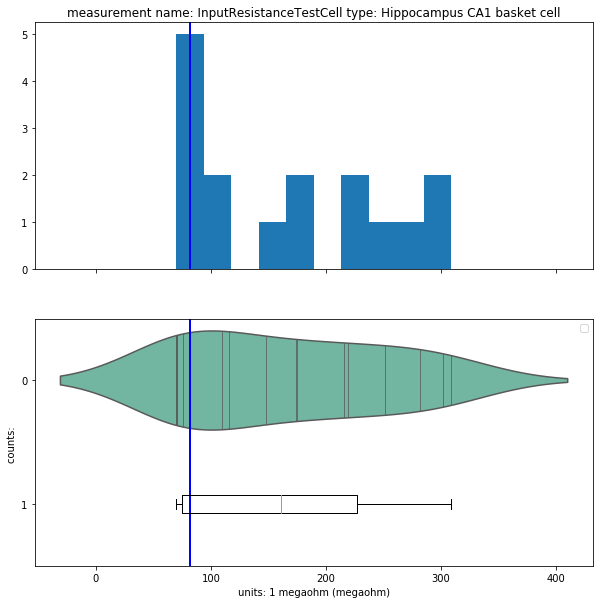
\includegraphics[scale=0.45]{notebooks_converted/needata_thesis_files/needata_thesis_5_5}
%\caption{Model parameterization of the brian2 simulator with the customization: interpolated spike height, forced to be above $0mV$}

  \label{fig:sub1}
\end{subfigure}%
\begin{subfigure}{scale=0.5}
  \centering
  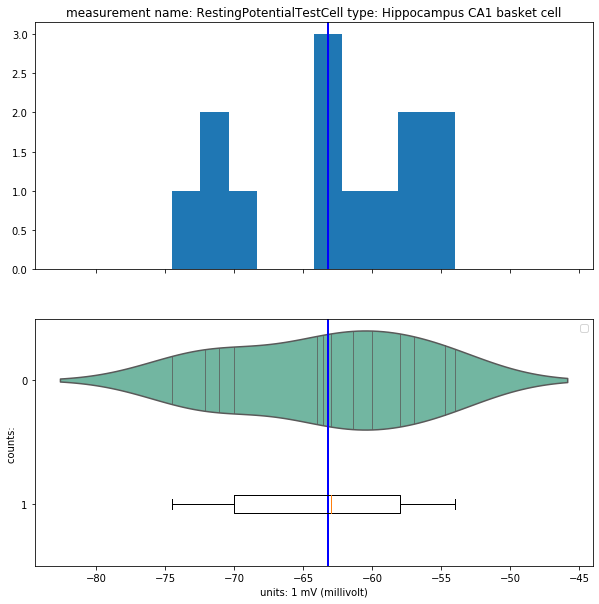
\includegraphics[scale=0.45]{notebooks_converted/needata_thesis_files/needata_thesis_5_6}
    
    %\caption{Default model parameterization of the custom written integrator}
  \label{fig:sub2}
\end{subfigure}

\begin{subfigure}{scale=0.5}
  \centering
      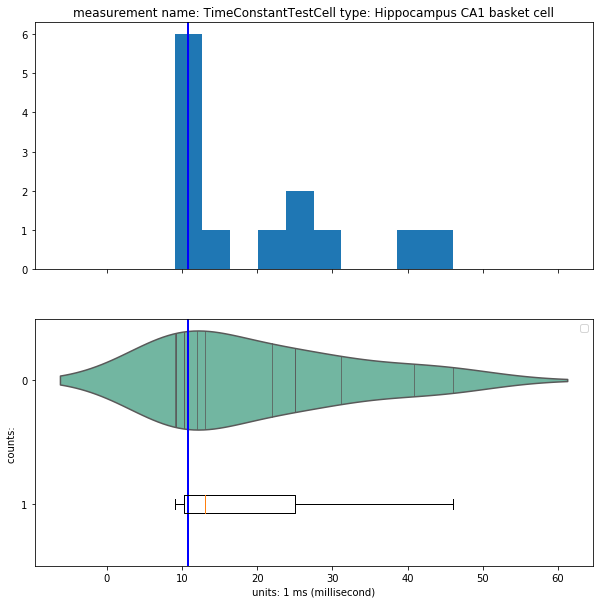
\includegraphics[scale=0.45]{notebooks_converted/needata_thesis_files/needata_thesis_5_7}
      %\caption{Default model parameterization of the custom written integrator}
  \label{fig:sub2}
\end{subfigure}

%\caption{Comparison between two Adxaptive Exponential Implementations}
\label{fig:test}
\end{center}
\end{figure}

\end{comment}

    
    %\begin{center}
    %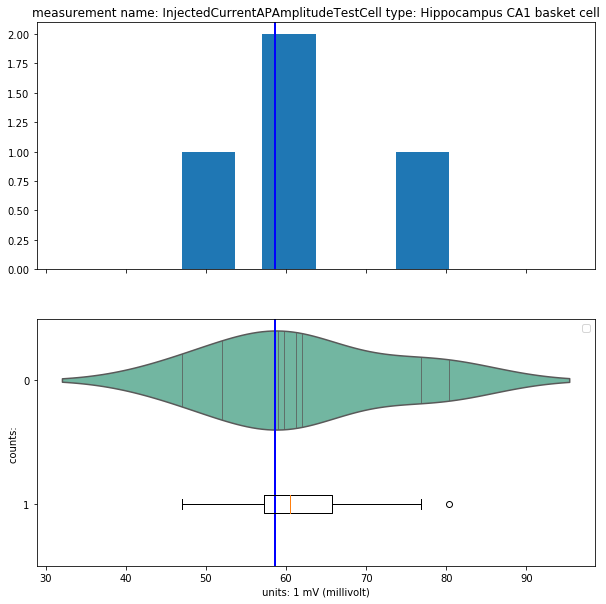
\includegraphics[width=0.7\linewidth]{notebooks_converted/needata_thesis_files/needata_thesis_5_8}
    %\end{center}
    %
    
\begin{figure} 
    \begin{center}

   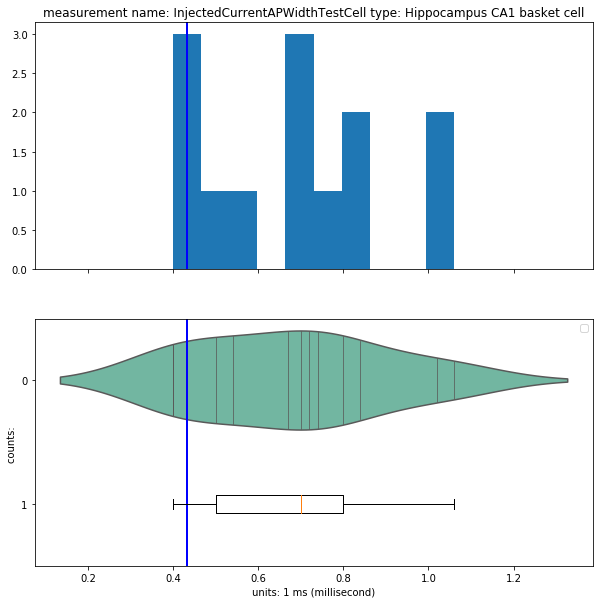
\includegraphics[scale=0.45]{notebooks_converted/needata_thesis_files/needata_thesis_5_9}
   \caption{The Action Potential Width of the Hippocampus CA1 basket cell possibly has either an underlying uniform distribution or a multimodal distribution. Since the samples are few, the true distribution is unknown. If the distribution is uniform the gaps in the distribution, that give the histogram a multimodal appearance, as the sample size is lower enough that such gaps may only represent missing samples.}
    \end{center}

\end{figure}
    { \hspace*{\fill} \\}

   \begin{figure}   
\begin{center}

   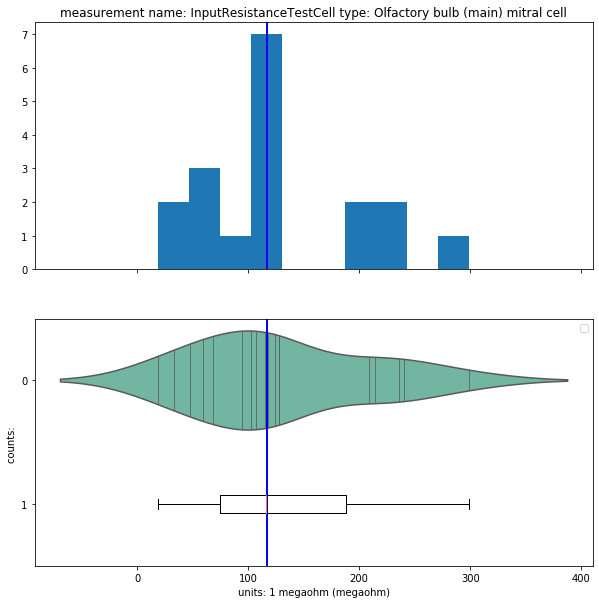
\includegraphics[scale=0.45]{notebooks_converted/needata_thesis_files/needata_thesis_5_21}
         \caption{Input resistance of the Olfactory Mitral cell showed some tendency towards underlying bi-modal distribution, however the second block of histogram bins, centered around $200-300pA$ only contains approximately $5$ samples}
\end{center}

   \end{figure}
   
\begin{figure}  
\begin{center}     

  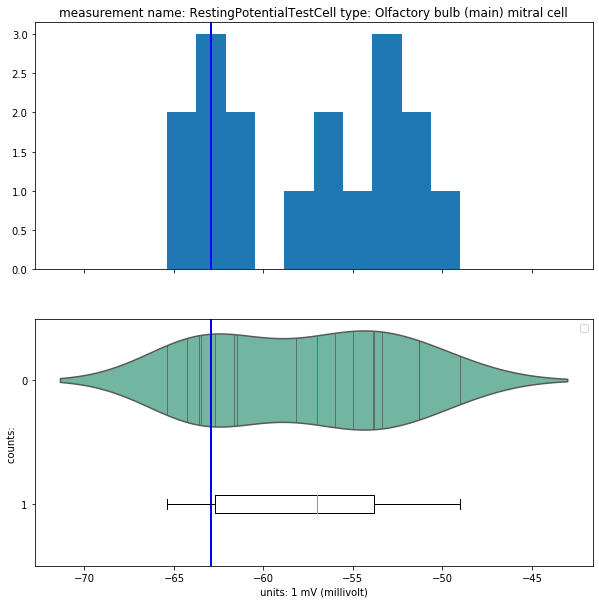
\includegraphics[scale=0.45]{notebooks_converted/needata_thesis_files/needata_thesis_5_22}
      \caption{Among different measurement sources of neuroelectro data, the resting membrane potential of the Olfactory Mitral cell, showed the greatest tendency of an underlying bi-modal distribution
      In the top panel of this plot we see a binned histogram of Resting membrane potential in the olfactory mitrall cell      
      }

\end{center}     
\end{figure}



\begin{figure}
  \centering
  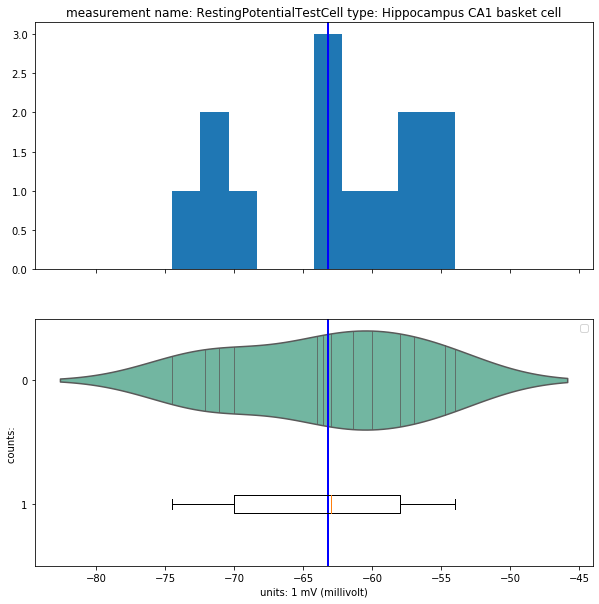
\includegraphics[scale=0.45]{notebooks_converted/needata_thesis_files/needata_thesis_5_6}
    
    %\caption{Default model parameterization of the custom written integrator}
  \label{fig:sub2}
\end{figure}

%    \begin{center}
%   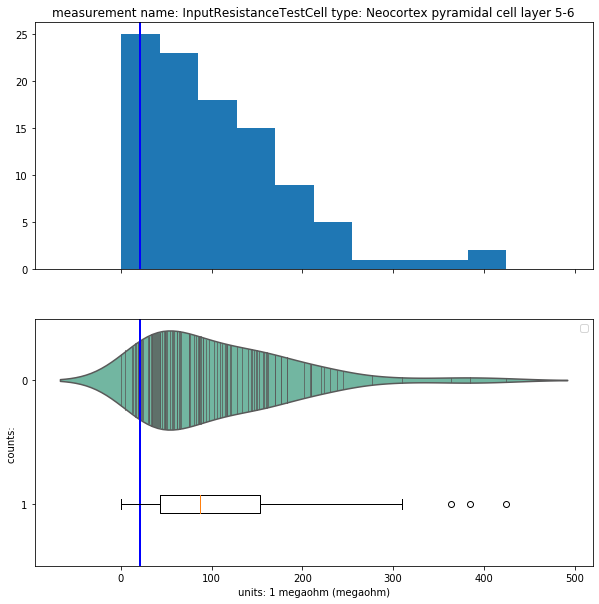
\includegraphics[width=0.7\linewidth]{notebooks_conver%ted/needata_thesis_files/needata_thesis_5_13}
%    \end{center}
    
    
%    \begin{center}
%    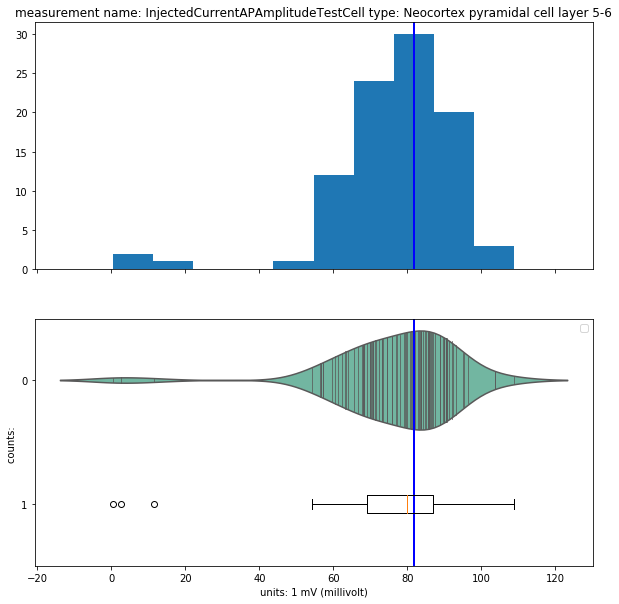
\includegraphics[width=0.7\linewidth]{notebooks_converted/needata_thesis_files/needata_thesis_5_16}
%    \end{center}

\begin{figure}
\begin{center}

     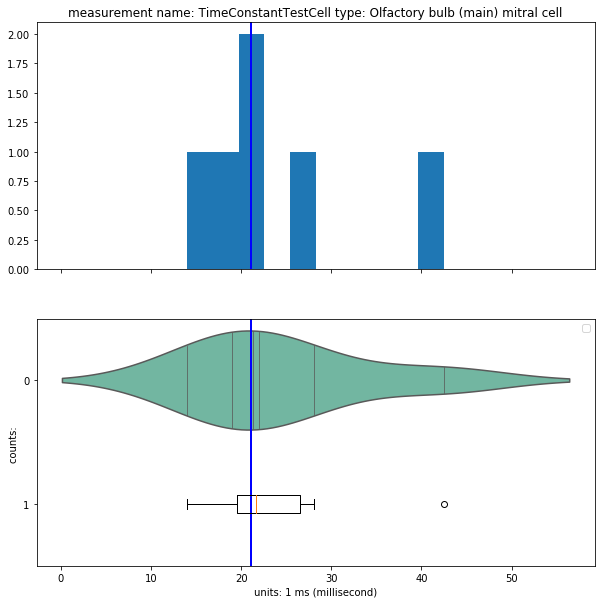
\includegraphics[scale=0.5]{notebooks_converted/needata_thesis_files/needata_thesis_5_23}
\caption{In the top panel of this plot we see a binned histogram of Neuro electro spike width measurements in the CA1 basket cell Neuron, in the bottom panel we see a violin plot, and a box plot of the same data. In both top and bottom panels, the mode is of the distribution is denoted by a blue vertical line. In this way the mode of the data distribution can be compared to the mean in the box plot. Often modes, and means of the measurements disagree, as they do in the case of CA1 basket cell spike widths. When consulting NeuroElectro measurement, a very common distribution shape is one which is possibly uniform, or multi-modal. It is perhaps obvious but worth noting that a uniform distribution, is not well described by a normal distribution. Under a normal distribution a range of measurement values are equally likely to occur.}
\end{center}

\end{figure}

   

\subsubsection{Reliable Optimization Depends on tractable Convex Errors used that can Guide Optimization}


Theoretically the largest possible number of constraints would be applied to optimization, because each constraint may provide additional information about the error surface, and may more rapidly exclude great volumes of the solution space. Despite this observation, except in good luck, a successful optimization recipe will not involve the use of all available fitness criterion. This makes the task of model-data fitting far from automatic, in fact human intervention is needed because, not all error signals can be informative guides. 

%\begin{itemize}
    %\item[-] Although there is a large variety of possible errors to use, its rarely a good idea to use all of these errors at once.
    
    One type of error that is an unreliable guide, is one who, by some minor aspect, contains a reference point, that is construed relative to each different model parameterization. In an effort to make computer code run without error, under very many different possible conditions, it is tempting to make model measurements that are not objective and unchanging between models. 
    
    A $V_{T}$ threshold my be computed as $(\frac{1}{10})\frac{dV_{M}}{dt}$.
    
    If a neuron model has a spike height below $0mV$, one may be tempted to set a spike detectors threshold as a multiple of $\mu_{V_{M}} - \sigma_{{V_{M}}}$, the mean $V_{M} -$ the standard deviation of the $V_{M}$. This would certainly detect spikes with peaks below $0mV$, and it would work for a wide variety of models too, however, the problem is that because the measurement has a dependency that is relative its self, it is less able to objectively assess waveform differences between  different models.\\
    \\
    For example spike width measurements, need to know the time when the peak of a spike occurred such that it can measure the time between $V_{T}$ and $V_{peak}$. If the method for obtaining spike time, adjusts itself to accommodate model specific differences, in the case when spike time is the same between models, some models will say a spike occured a bit later, and others a bit earlier, resulting in an unwarranted difference between measurements, which will misguide optimization. The problem can be compounded because other measurements can depend on this measurement, such as spike height, spike width, and $V_{T}$, all of these depend on the spike detection threshold. Which is now not really constant between models.\\
    \\
    Another cause of misguided errors may involve the recalculating the Rheobase current injection value between different models, there is some error associated with approximating the rheobase current. What is desired is to ascertain the minimal current injection amplitude, which would cause only one spike to fire, but because there is not much time to exhaustively test smaller and smaller values of current amplitude (due to the exploration, exploitation dilemma), one will always settle for an over estimate, one that is somewhere between enough current to cause one or two spikes. The size of this error will vary between models. In addition to this finite precision error, a measurement that is relative to each model, and not objective between models, is a bad idea for the same reason as the model specific measurement for $V_{T}$.\\
    \\
    Spike amplitude will be bigger for some models at their rheobase calculation than other models, especially between models of different input Resistance. Input Resistance will succeed in attenuating greater amplitudes of applied current, however, if a the current succeeds at provoking a spike, the voltage deflection will have a larger peak because of Ohms law: $V=IR$. In this case $V_{M}$, specifically the peak of $V_{M}$ deflection is proportionate to current injection amplitude. So models with different amounts of input resistance will also differ in the peak of the rheobase current injection. However because rheobase is re-calculated per model and because there is finite precision in the rheobase error calculating software it is possible that there will be small regions of error surface, that less accurately encode this relationship.\\
    \\ 
    The situation then compounds when other measurements are taken which depend on rheobase values. An alternative exists where, you sample an error surface using a fixed amount of current preferably at the observed Rheobase current of an experimental cell you are investigating. This would make "Rheobase" a hard constraint, models either spike at the prescribed current, or they don't. Meaning many models are instantly eliminated only because they failed to match Rheobase value, and models that pass this Rheobase test, may score poorly across every other NeuronUnit criteria.
    
    The appeal of applying rheobase as a soft constraint, is it better solutions should be possible, if models are allowed to perform badly on the rheobase score and good at all other criteria, however, there may be other ways of achieving this.
    
    When applying a fixed rheobase current across many different models only neurons that fail to spike need to be excluded, neurons that fire multiple spikes can still have their spike shapes measured. Additionally, it would be acceptable to run different optimization batches, at different current injection amplitudes, and to federate scores between batches of different current amplitude. The reason why batches need to remain seperate, is that, its only important that error surfaces are convex within the one optimization process. Its okay if two different processes are using different surfaces, as each is blind to the others internal error surface.\\ 
    \\
    %The down side to this approach, is that by distributing the optimization job into batches, it begins to take on an exhaustive nature, and it is not really known, how many current levels would need to be independently explored to achieve good results.\\
    \\
    A different approach was also utilized, where three static quantities of current amplitude $(300pA, 450pA, and 900pA)$ was applied uniformly to all sampled model parameterizations. 
    Another approach, was explored were larger volumes of the solution space were immediately excluded, by way of fixed current.
    %more exclusively
    be to apply a large enough current to invoke spiking in most neurons, and to measure the wave form shape of just one or two spikes in a the resulting spike train.
    
    \subsubsection{Error signals derived from threshold calculations}
    %\begin{itemize}
    %\item[-] 
    A suite of NeuronUnit tests contained two threshold dependent measurements. These were spike half-width, spike height. The treshold was also used to comprize a NU test, so in total three $V_{T}$ measurements were used.
    
    %\item[-] 
    (Ephysiology Feature Extraction Library \cite{EFEL}) EFEL, Allen SDK, and Druckman all contain independently written algorithms for ascertaining modelled neuron $V_{T}$ thresholds calculation code. In all three feature extraction pipelines $V_{T}$ is computed by taking derivative of $V_{M}$
    %\end{itemize}
    
   Another related pitfall is the relationship between the number of free dimensions in the optimization problem versus the number of reliable errors used to constrain the optimization process.
   
   Genetic algorithms are known as derivative free optimizers, since the derivative of the error surface is not explicitly calculated, and genetic algorithms have properties that make them robust against local minima. However, just like in gradient descent, genetic algorithms act on information in the error surface. Although genetic algorithms are resilient against local minima, but they are still misguided by unfortunately positioned local error wells. For this reason Rastrigrins function is used to benchmark the performance of genetic algorithms.\\
   \\
   Rastrigins function has convexity in two scales. On the larger scale the surface has a convex property, on the small scale the function is uniformly pocked with minima wells. Inorder for the GA to optimize Rastrigins function it must be able to exploit the global information of the error surface, and simultaneously the genes will often converge for generations in the minima, but they won't get stuck there because mutation and cross-over will drive the GA to test other less optimal solutions.\\
   \\
   %\begin{figure}
  %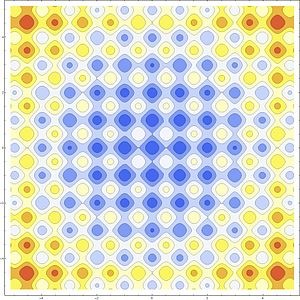
\includegraphics[]{figures/rastagrind.jpg}
  %\caption{}
   %\end{figure}
   
   It is worth noting that although Rastrigrins function is challenging it does not the present the worst gradient to learn from. Worse than Rastrigrins function, are functions that on a large scale are flat, but on the smaller scale contain a high density ripples.
   but lacks this global convex trend, excepting for an abrupt and localised descent to the optima.\\ 
   \\
   Without some first prior knowledge of the error surface, a likely outcome is to attempt optimize on uninformative surfaces. If an uninformative surface is applied, it does not mean that the genetic algorithm will not succeed, it only means that the performance of the GA may be only marginally better than random sampling, or exhaustive search of the error surface.\\
   \\
   Random sampling, sounds bad, however, if the best random solution is digitally stored, and the number of samples applied is less than the possible number of samples in an exhaustive search, random sampling may better resolve the exploitation/exploration dilemna than both gradient descent, and exhaustive search.
{ \hspace*{\fill} \\}      

In the figures below, I describe the spectrum of error surface quality.
\begin{figure}
\centering
\begin{minipage}{.5\textwidth}
  \centering
     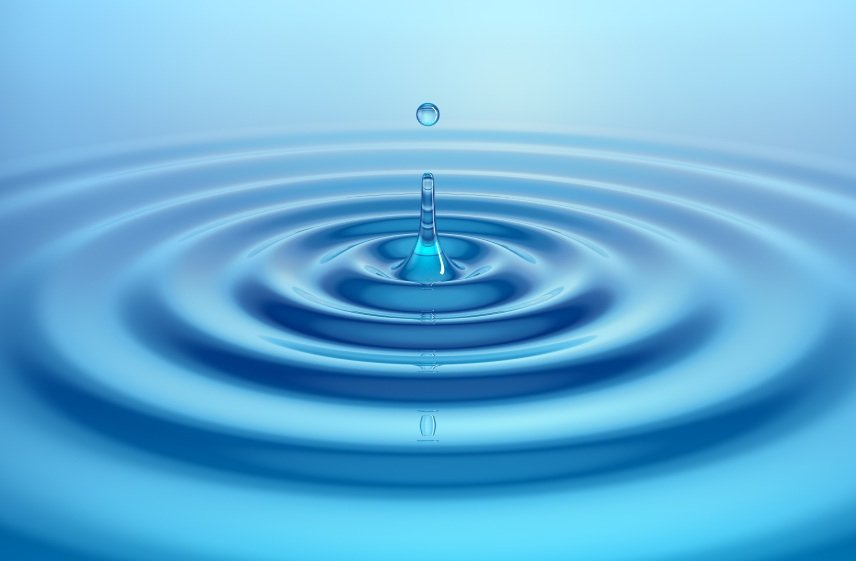
\includegraphics[scale=0.65]{figures/pond_ripple_surface.png}
     \captionof{figure}{In the case of pond ripples the cost function is defined so that the maxima is the optimal location on the surface. Ripples on a body of water are more challenging to optimize, as the water surfaces are approximately flat on the large scale, yet on the small scale maximas will be temporary preoccupy the GAs learning, but outside of those peaks, there is little large scale information to utilize. }
      
      \label{fig:test1}
    \end{minipage}%
    \begin{minipage}{.5\textwidth}
      \centering
      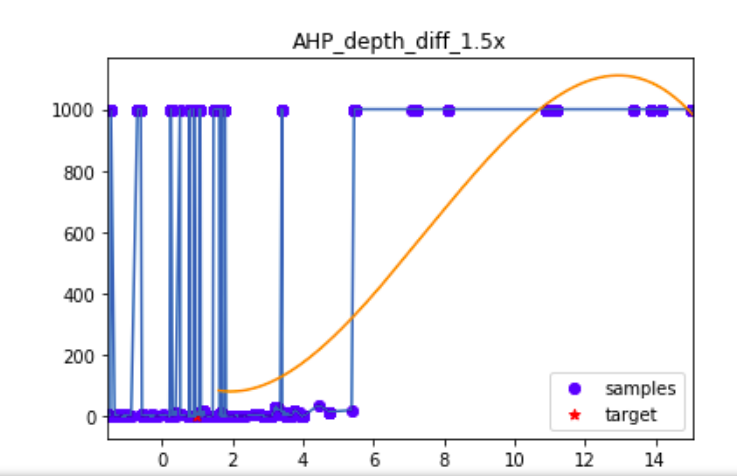
\includegraphics[scale=0.85]{figures/parameter_b_hopeless_surface2.png}
      \captionof{figure}{Similarily parameter b was slowly varied in the Izhikevich model while all other parameters where held constant, the AP1 begin voltage (threshold), was computed for each different model parameterisation of \emph{a}, this resultd in a highly rippled error surface, densely populated by local minima, and with only a very shallow global convex shape}
      \label{fig:test2}
    \end{minipage}
\end{figure}


% Note Help wanted making a professional version, of this known to be unattractive draft/concept figure.
\begin{figure}
\centering

      \label{fig:test1}
    \begin{minipage}{.5\textwidth}
      \centering
      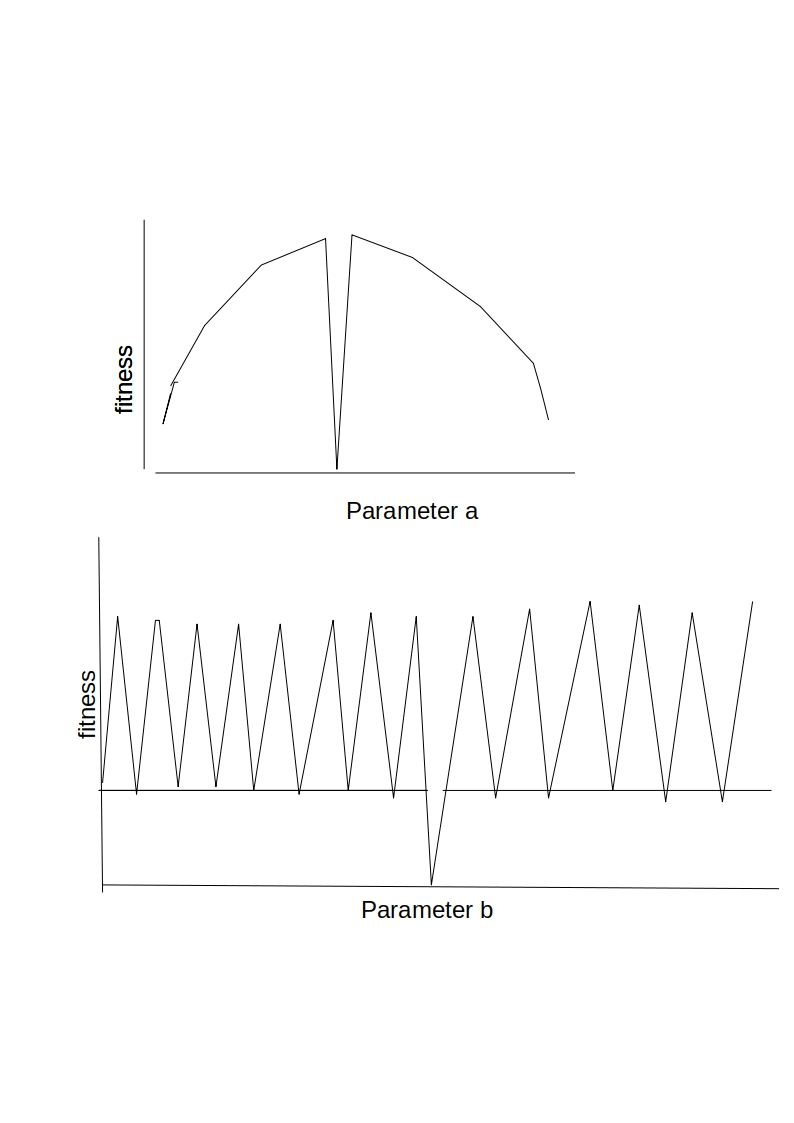
\includegraphics[scale=0.85]{figures/worst_error_surfaces.jpg}
      \captionof{figure}{Rastrigrins function describes a challenging error surface, but one with learnable global features that a genetic algorithm can exploit. It's important to note that there are much worse error surfaces, and these may show up in practice. The first type has actively misleading local and global information. In this context learning is a disadvantage, if the optimizer "learns", then it actually slows obtaining an optimal solution. The second type of error surface (actually a 1D (and upside down) cross section of the 2D pond picture, only actively misleads locally, globally it simply contains no helpful global information. Learning will not be of any assistance in obtaining the optima, but also learning won't actively be a disadvantage either, the Genetic Algorithm, will simply behave as a random sampling/testing algorithm, the GA will find the optimum in time, but possibly not as quickly or reliably as exhaustive search would. The second figure is a cross section of the pond ripple argument}
      \label{fig:test2}
    \end{minipage}
\end{figure}

\begin{figure}
\centering


    
    \begin{minipage}{.5\textwidth}
      \centering
      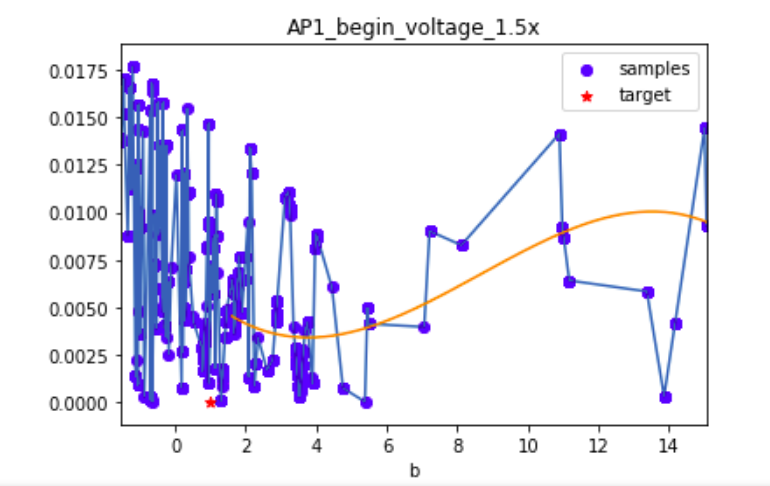
\includegraphics[scale=0.85]{figures/parameter_b_hopeless_surface.png}
      \captionof{figure}{Similarily parameter b was slowly varied in the Izhikevich model while all other parameters where held constant, the AP1 begin voltage (threshold), was computed for each different model parameterisation of \emph{a}, this resultd in a highly rippled error surface, densely populated by local minima, and with only a very shallow global convex shape}
      \label{fig:test2}
    \end{minipage}

    \begin{minipage}{.5\textwidth}
      \centering
      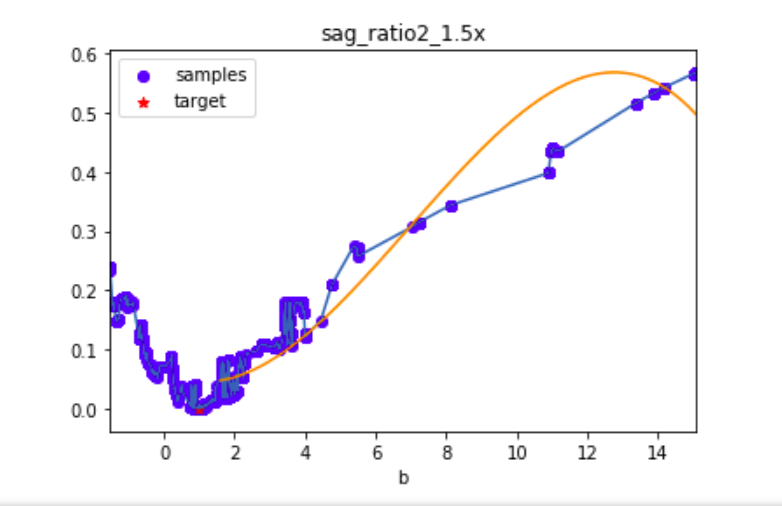
\includegraphics[scale=0.85]{figures/parameter_b_friendly_surface.png}
      \captionof{figure}{This is an example of a useable and tractable error surface, it has learnable global and local information, as long as not all error surfaces in the multiobjective collection of constraints, this surface is likely to be a valueable addition to the optimizer suite}
      \label{fig:test2}
    \end{minipage}


\end{figure}



     
   When considering 2D relationships between single parameters and single objective functions, ideally each objective function might contribute helpful information, that on mass boosts the total amount of helpful information. For-instance some 2D error mappings, may contain one or more local minima, but in the same region a different error mapping could lack the well, meaning that at least one out of two error functions contribute incentive to stride across a minima. The mapping that contains wells, might still be useful to guide optimization, as it may also lack minima in regions were the counterpart has them, additionally the counterpart mapping may have regions of $~0.0$ gradient where the other mapping contains significant gradient.\\
   \\
   It is almost impossible to make progress without some prior knowledge of the error surfaces, as knowledge of the error surface is a prerequisite for constraining optimization. Not all surfaces, provide equally useful information. There are spectrums of surface quality between convex traingular or parabolic depressions acting as the best solution surfaces, and flat functions 
   $NDIM:NOBJ$
   
   Ideally each extra $NOBJ$  

%\end{itemize}
  
\subsubsection{Parallel Rheobase Solver}

The Rheobase determination algorithm was in fact a specific instance of a more general type of algorithm, one that finds the current injection that causes a pre-determined number of spikes.

\begin{figure}    
  \begin{center}
  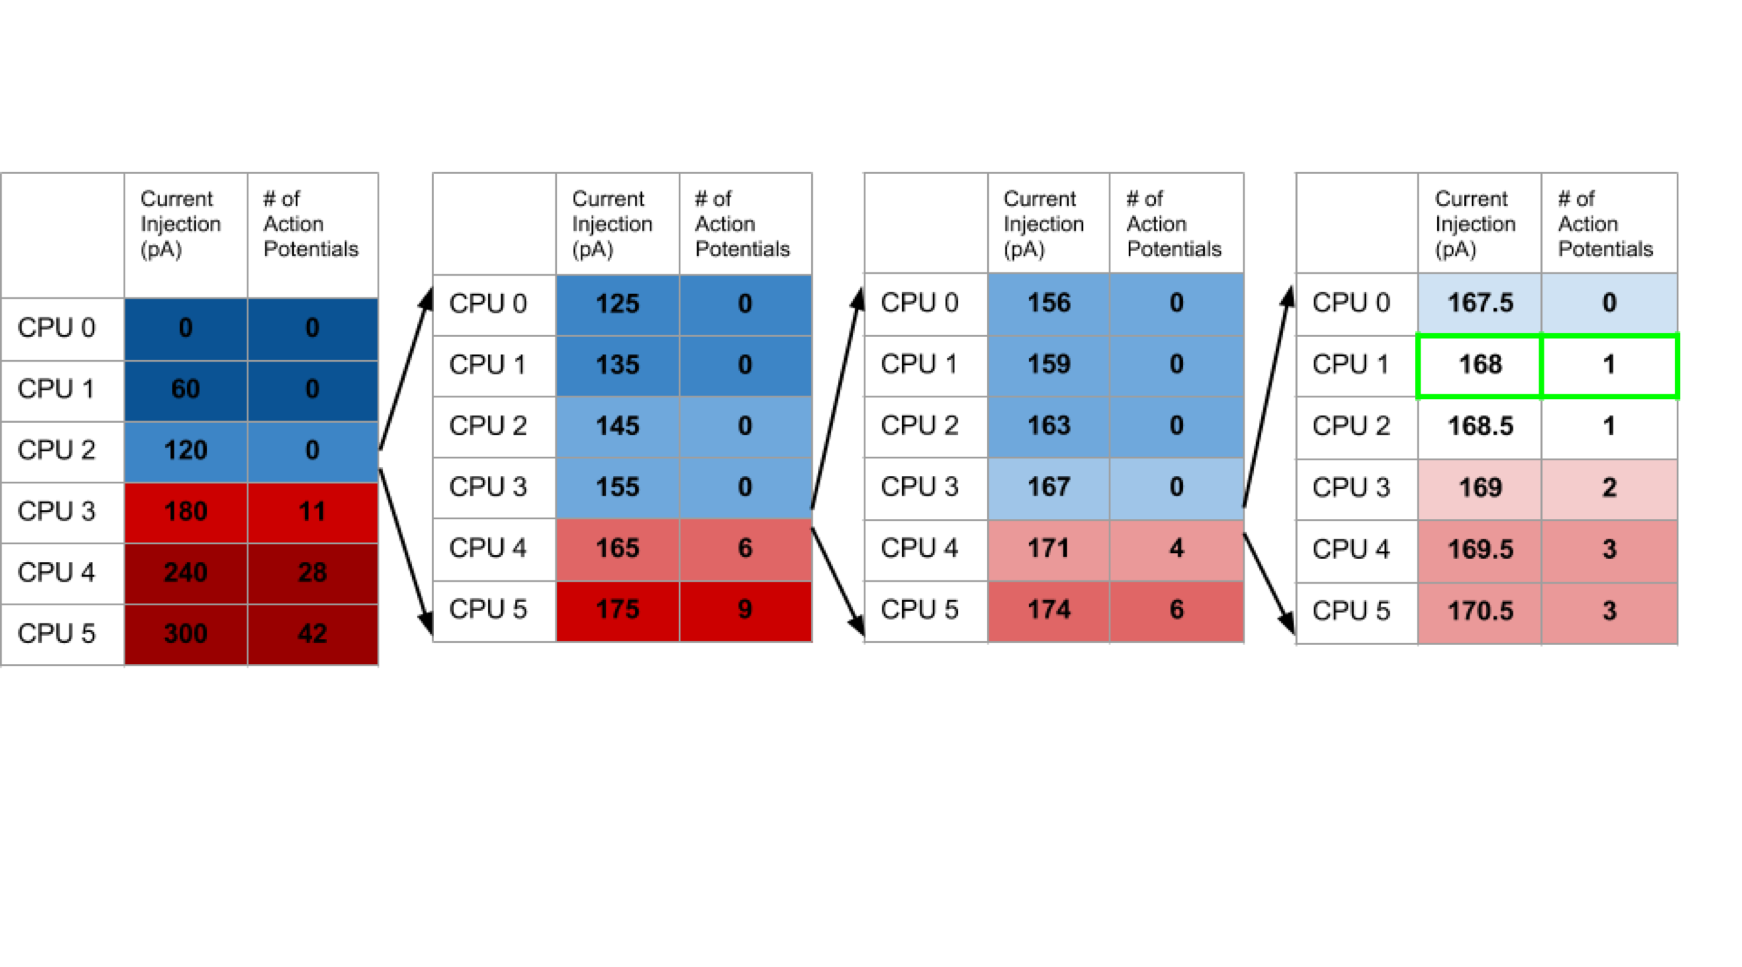
\includegraphics[width=0.7\linewidth]{{figures/rheobase_algorithm.png}}
    \caption{We developed a generic algorithm which took models, and found the minimal current injection value that would cause only one spike. The normal structure of this algorithm is a binary search, however we modified the algorithm so it would map onto multiple processors at once. This lead to significant speed ups for multicompartment NEURON models}

  \end{center}
\end{figure} 
    
Below I show that for multi-compartment neuron models using a parallel Rheobase algorithm adds a significant speed up to rheobase solution evaluation. It
is important to consider that determinig rheobase usually involves
between 10-35 model simulations at different current injection
strengths. Whereas the remaining error score calculations only involve
at most one model evaluation each. Consider an optimization problem where
there are only eight error scores to calculate, and four of the eight
errors are for non spiking simulations of less than 500ms, a rheobase
simulation is for 1200ms, and it involves both non-spiking and
multi-spiking behavior. Multi-spiking models take longer to simulate
than non spiking and single spiking models for the simple reason that $\frac{dV_{M}}{dt}$ changes rapidly and solvers that are capable of variable time steps, will not be able to exploit sparse sampling in these rapid changes of  $\frac{dV_{M}}{dt}$. In this particular
instance where finding the unique rheobase value for each different gene
is important, that rheobase determination is the biggest computational
bottleneck.

It is also important to consider that the speed of model simulation is
often determined by the exact parameterization of the model in question.
During optimization parameterization frequently changes. Multi-spiking
models that are slower to evaluate are frequently sampled by a genetic
algorithm optimizer.

parallel Rheobase search time NEURON  $4.8$
serial Rheobase search time NEURON  $18.7$
Approximate speed up $\times 3.9$

Brian2 adaptive Exponential model   
elapsed serial:  $0.7914438247680664$
elapsed parallel: $ 0.2590057849884033$
speed up parallel:   $\times 3.0$

Algorithm was able to speed up this slow NEURON unit code. $ \frac{73}{19} $ represents a substantial speed up. of about 3.8. This is consistent with previous work

%$ array(51.79317142) * pA$

 
\section*{Technical Details of the Optimizer}
Experimental Recording Features from Neuroelectro. And some from the Allen Celltypes data-base.

%It was possible that some selections of experimental data, might be supurious or compromised in some way.  

The algorithms IBEA and NSGA2 seem to result in different optimization convergence speeds, and similar solution quality, but this varied in a problem specific manner. Generally it was found that IBEA produced better results faster, although, often it could produce solutions that were significantly dominated in one error score.

Typical model parameters were number of generations $(NGEN=150$, population size:$MU=25$. There was plenty of opportunities to change these parameters,  values of $NGEN$ and $MU$ as small as $(10,10)$ were tolerable under some limited circumstances, and also multiobjective optimizations with $NOBJ>25$ demanded $NGEN=200$, and $MU=50$ in order to unearth good results.

%\item Python, NeuroUnit, 

\subsection{Model/Test combinations}

Contrast with other optimization approaches:
There are two different strategies, one strategy involves evaluating goodness of fit, only at one current injection strength for every gene. Another approach is a bit more generous, in that, rather than allowing models to instantly fail to evoke a spike at the appropriate current injection, that models specific rheobase value is found, and all other tests are evaluated at the current injection value. The consequence of accomodating poorer fits on the Rheobase test, is allows models to compete on the other seven or more different fitness criteria.

\subsection{Elephant Test Suite}
At a count of eight tests (five useable) the elephant derived suite was relatively compact. The elephant tests suite is concerned with core ephysiology measurements, the particular measurements chosen were important because, for example capacitance, and input resistance directly affect the evolution of reduced model governing equations. Taken as a collection these ephysiological properties as a collection also determine spiking waveform shape. 

Capacitance, Rheobase, Time Constant, Input Resistance, Resting Potential

%\item 
Result It when models were fitted using the following measurements alone, the resulting models were also fitted to spike half-width, arguably because the membrane time-constant, and membrane capacitance together encode spike-half width.

\subsection{Electrophysiology Feature Extraction Library}

Many of the EFEL measurements, and Allen SDK Feature measurements pertain to spike train statistics, because model fitting to spike train statistics is a productive and well understood domain, we did not utilize spike train statistics in model fitting. Instead EFEL spike shape and electrophysiology measurements were applied.\\
\\
Through trial and error experimentation the following EFEL features were demonstrated to result in helpfull and tractible error surfaces. In simulated constraint paradigms using the aforementioned EFEL fitness criteria, lead to recovery of optimal models. This finding did not apply to the entire collection of EFEL features however.\\
\\
In a large scale analysis of variance between models and data see section large\_scale\_variance

%\href{run:./RESULTS_large_scale_variance}{RESULTS_large_scale_variance}

\begin{comment}
\centering
\begin{tabular}{l}
\toprule
{}  freature  \\
\midrule
AHP\_depth\_abs\_3.0x \\
 sag\_ratio2\_3.0x \\
$ ohmic_input_resistance\_1.5x$ \\
$ sag_ratio2\_1.5x$ \\
$ peak_voltage\_3.0x$ \\
$ peak_voltage\_1.5x$ \\
$ voltage_base\_3.0x$ \\
$ voltage_base\_1.5x$ \\
$ Spikecount\_1.5x$ \\
$ Spikecount\_3.0x$ \\
$ ohmic\_input\_resistance\_vb_ssse_1.5x$ 
\bottomrule
\end{tabular}
\end{comment}

%\item 
Unlike in BluePyOpt \cite{bluepyopt} and Allen Institute optimization workflows \cite{gouwens} rheobase current injection was applied is a soft constraint. However, this work differs from other work in that rheobase current injection was found for every different model paramerisation.
%\item 
Rheobase value as a soft constraint. This means that current injection values are a variable model parameter. The exact value of current used is determined via exploring the model response to current injections of varying amplitude. The exact value, its value is determined by other model parameters.

spike shape measurements and error functions. We used a set of 8 different experimental measurements NeuronUnit.


\begin{figure}
\begin{center}
	\includegraphics[0.65]{figures/normal_distribution}
    \caption{As discussed in the introduction, Error functions were evaluated with the assistance of a library: \emph{NeuronUnit} 
    were based on finding a normal distribution on electro physiology measurements, 
    and then measuring model outputs and mapping the model behavior onto
     a place on the experimental normal distribution. Scores that where closer to the
      experimental mean where deemed to be low in error.
	Z-scores obtained via NeuronUnit can be thought of as  }
	%\label{figure\arabic{figurecounter}
	
\caption{Caption}
\end{center}
	
\end{figure}
